%\documentclass[pdflatex,11pt]{../aghdoc}
\documentclass{../aghdoc}               % przy kompilacji programem latex
\usepackage[polish]{babel}
\usepackage[utf8]{inputenc}

% dodatkowe pakiety
\usepackage{enumerate}
\usepackage{listings}
\lstloadlanguages{TeX}

\lstset{
  literate={ą}{{\k{a}}}1
           {ć}{{\'c}}1
           {ę}{{\k{e}}}1
           {ó}{{\'o}}1
           {ń}{{\'n}}1
           {ł}{{\l{}}}1
           {ś}{{\'s}}1
           {ź}{{\'z}}1
           {ż}{{\.z}}1
           {Ą}{{\k{A}}}1
           {Ć}{{\'C}}1
           {Ę}{{\k{E}}}1
           {Ó}{{\'O}}1
           {Ń}{{\'N}}1
           {Ł}{{\L{}}}1
           {Ś}{{\'S}}1
           {Ź}{{\'Z}}1
           {Ż}{{\.Z}}1
}

%---------------------------------------------------------------------------

\author{Tomasz Kasprzyk, Daniel Ogiela, Jakub Stępak}
\shortauthor{T. Kasprzyk, D. Ogiela, J.Stępak}

\titlePL{System obliczający wyniki wyborów dla uogólnienia systemu k-Borda}

\shorttitlePL{System obliczający wyniki wyborów dla uogólnienia systemu k-Borda} % skrócona wersja tytułu jeśli jest bardzo długi

\thesistypePL{Dokumentacja użytkownika}

\supervisorPL{dr hab. inż. Piotr Faliszewski}

\date{2016}

\departmentPL{Katedra Informatyki}

\facultyPL{Wydział Informatyki, Elektroniki i Telekomunikacji}

\setlength{\cftsecnumwidth}{10mm}

%---------------------------------------------------------------------------

\begin{document}

\titlepages

\tableofcontents


%----------------------------------------------------------------------------
\chapter{Wstęp}
\label{cha:wstep}

Niniejszy podręcznik opisuje sposób użytkowania systemu \texttt{Election Computing System}, powstałego w ramach pracy inżynierskiej realizowanej na Akademii Górniczo-Hutniczej w Krakowie.

System umożliwia obliczenie wyników wyborów w uogólnionym systemie wyborczym k-Borda. Szczegóły na temat tego systemu wyborczego można przeczytać w Przewodniku po projekcie.


\chapter{Instrukcja uruchomienia systemu}
\label{cha:uruchomienie}

Działającą aplikację można przetestować na stronie: \\ \url{https://election-computing-system.herokuapp.com}. 

Ze względu na ograniczenia na ilość rekordów w bazie danych narzucone przez darmową wersji Heroku, nie będzie można dodać tam zbyt „dużych” wyborów (ograniczona jest liczba głosujących i kandydatów). Aby korzystać z pełnych możliwości aplikacji, należy uruchomić ją na własnym komputerze. Dalsza część tego rozdziału opisuje jak to wykonać.

\section{Przygotowanie środowiska}
\label{sec:srodowisko}

\subsection{Język}
\label{subsec:jezyk}

System jest aplikacją internetową opartą o framework Django napisaną w języku Python 2.7.
Aby uruchomić aplikację, należy uprzednio zainstalować na swoim komputerze interpreter Pythona.

\subsection{Repozytorium}
\label{subsec:repo}

Repozytorium projektu znajduje się pod adresem: \\ \url{https://github.com/jakubste/election-computing-system}.
Projekt należy sklonować używając programu Git 
\begin{lstlisting}[language=bash]
$ git clone git@github.com:jakubste/election-computing-system.git
\end{lstlisting}
lub ściągnąć jako ZIP bezpośrednio z GitHuba i rozpakować w wybranym miejscu.

\subsection{Biblioteki}
\label{subsec:repo}

Do instalacji bibliotek zaleca się używanie mechanizmu \texttt{virtualenv}, który separuje środowiska uruchomieniowe dla poszczególnych projektów. Autorzy projektu zalecają też dla wygody wykorzystanie \texttt{virtualenvwrapper}'a. Do instalacji bibliotek można użyć programu \texttt{pip}.
Informacje o wymaganych bibliotekach są zawarte w pliku \texttt{requirements.txt}.
\begin{lstlisting}[language=bash]
$ mkvirtualenv inz
$ pip install -r requirements.txt
\end{lstlisting}

\subsection{Baza danych}
\label{subsec:database}

Aplikacja domyślnie jest skonfigurowana do użycia z bazą danych dostarczaną przez Heroku (PostreSQL). Dla ułatwienia zostanie przedstawiony sposób konfiguracji z użyciem SQLite3. O konfiguracji dostępu do innych baz danych można przeczytać w dokumentacji Django. 

W celu skonfigurowania swojej bazy danych należy w katalogu \texttt{ecs} utworzyć 
plik \texttt{local\_settings.py} i umieścić tam następujący kod:

\begin{lstlisting}[language=Python]
from settings import *

DATABASES = {
   'default': {
       'ENGINE': 'django.db.backends.sqlite3',
       'NAME': os.path.join(BASE_DIR, 'db.sqlite3'),
   }
}
\end{lstlisting}

Następnie w katalogu głównym programu należy wykonać polecenie:
\begin{lstlisting}[language=bash]
$ ./manage.py migrate
\end{lstlisting}


\section{Uruchomienie serwera}
\label{sec:serwer}

W tym momencie aplikacja powinna być gotowa do działania.
W katalogu głównym programu należy wykonać polecenie:
\begin{lstlisting}[language=bash]
$ ./manage.py run_server
\end{lstlisting}

Po otworzeniu w przeglądarce internetowej adresu:
\begin{lstlisting}
http://localhost:8000/
\end{lstlisting}
powinna pojawić się strona podobna do tej:


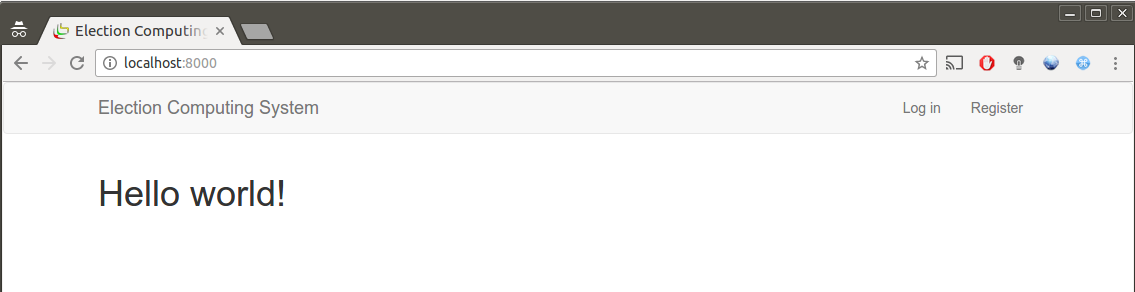
\includegraphics[width=0.8\textwidth]{pics/first_view.png}


\subsection{Metoda k-Borda}
\label{subsec:metoda_k_borda}

Rozszerzenie metody Bordy. Wynik, zamiast dla jednego kandydata, obliczany jest dla ciągu kandydatów. $f_{kB}$- funkcja zadowolenia z komitetu. Ciąg $(i_1,\dots, i_k)$- ciąg pozycji kandydatów

\paragraph{Przyklad}
$C={c_1,c_2,c_3,c_4}$ - zbiór kandydatów, 
$v=(c_2,c_1,c_4,c_3)$ - głos
Niech $k = 2$ (wybory $2$ spośród $4$)
$w=(c_4,c_3)$
Najpierw określamy pozycje kandydatów z komitetu $w$ w $v$:
$pos_v(w)=(3,4)$, zatem wynik komitetu w dla głosu v wynosi
$f_{kB}(3,4) = (3) + (4) = ||C|| - 3 ) + ( ||C|| - 4 ) = 1 + 0 = 1$


\subsection{Uogólnienie - system $\ell_p$ Borda}
\label{subsec:system_ell_p_borda}

Zanim wprowadzone zostanie pojęcie uogólnionego systemu k-Borda warto przypomnieć wzór na normę $\ell_p$

\subsubsection{Norma $\ell_p$}
\label{subsubsection:norma_ell_p}

$\ell_p(x_1,x_2,\dots, x_n) = \sqrt[p]{x_1^p+x_2^p+\dots+x_n^p},$ 


Wówczas, w uogólnionej wersji metody k-Borda, funkcja zadowolenia $f_{kB}$ zostaje uzależniona również od parametru $p$ z powyższego wzoru. Norma liczona jest z wyników według Bordy, $\beta(i)$. Wzór uogólniony funkcji zadowolenia przyjmuje zatem postać:\\
$f_{\ell_pB}(p,(i_11,\dots,i_k))=p[(i1)]p+[(i2)]p+...+[(ik)]p$


Systemy  k-Borda i Cahmberlin’a-Courant’a są szczególnymi przypadkami zdefiniowanego powyżej systemu $\ell_p$- Borda:\\
Dla $p = 1$, $l_1$\\
$f_{\ell_pB}(1,(i_1, \dots ,i_k)) = \beta(i_1) + \beta(i_2) + \dots + \beta(ik) = f_{kB}(i_11, \dots,i_k)$\\
Dla $p= \infty$,  $l_{\infty}={max}$\\
$f_{\ell_pB}(\infty,(i_1, \dots ,i_k))=\lim\limits_{p \to \infty} \sqrt[p]{\beta\left[(i_1)\right]^p+\beta\left[(i_2)\right]^p+ \dots +\left[\beta(i_k)\right]^p}=\max{\beta(i_1),\beta(i_2),\dots,\beta(i_k)} = \beta(i_1)=f_{CC}$

\section{Format danych wejściowych}
\label{sec:format_danych_wejsciowych}

\section{Szybkość i dokładność wykonywanych obliczeń}
\label{sec:szybkosc_i_dokladnosc_wykonywanych_obliczen}

\chapter{Opis modułów}
\label{cha:opis_modulow}


\bibliographystyle{alpha}
\bibliography{bibliografia}

\end{document}
